\documentclass[border=10pt]{standalone}
\usepackage{pgfplots}
\usepackage{siunitx}
\pgfplotsset{width=7cm,compat=1.8}
\usepgfplotslibrary{polar}
\pgfplotsset{myplot/.style={%
  clip=false, % needed for double line (last \addplot command)
  domain=0*pi:2*pi, % plot full cycle
  samples=600, % number of samples; can be locally adjusted
  grid=none, % display major and minor grids
  xtick={0,pi/2,...,2*pi},
  xtick align=outside,
  xticklabels={%
  $0$,  
  $\pi/2$,
    $\pi$,
    $3\pi/2$,
    $2\pi$
  },
  major grid style={black}, 
  yticklabel style={anchor=east}, % move label position
}}
\begin{document}
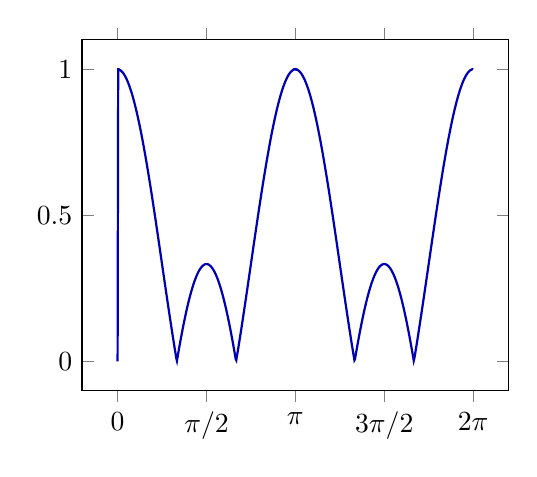
\begin{tikzpicture}

    \begin{axis}[%
      myplot]
      \addplot[mark=none,blue!70!black,thick]{1/3*abs(sin(deg(3*\x))/sin(deg(\x))};

                
      
      \end{axis}
\end{tikzpicture}
\end{document}